\documentclass[twoside,11pt]{article}

% Any additional packages needed should be included after jmlr2e. Note that jmlr2e.sty includes
% epsfig, amssymb, natbib and graphicx, and defines many common macros, such as 'proof' and
% 'example'.
%
% It also sets the bibliographystyle to plainnat; for more information on natbib citation styles,
% see the natbib documentation, a copy of which is archived at http://www.jmlr.org/format/natbib.pdf

\usepackage[utf8]{inputenc}
\usepackage{jmlr2e}
\usepackage{amsmath}
\usepackage{hyperref}
\usepackage{textgreek}
\usepackage{algorithm,algorithmic}
\usepackage{graphicx}
\usepackage{subcaption}
\usepackage{booktabs}
\usepackage{enumitem}

% Definitions of handy macros can go here
\newcommand{\dataset}{{\cal D}}
\newcommand{\fracpartial}[2]{\frac{\partial #1}{\partial  #2}}

\renewcommand{\algorithmicrequire}{\textbf{Input:}}
\renewcommand{\algorithmicensure}{\textbf{Output:}}

% Heading arguments are {volume}{year}{pages}{submitted}{published}{author-full-names}
\jmlrheading{Projects Spring \textquotesingle{}26}{2026}{1--12}{May 2026}{June 2026}
{Jonas Adomaitis, Tomas Giedraitis, Gedas Ber\v{z}inskas}

% Short headings should be running head and authors last names
\ShortHeadings{EEG functional data analysis}{Adomaitis, Giedraitis, Ber\v{z}inskas}
\firstpageno{1}

\begin{document}

\setlength{\parindent}{15pt}

\title{Flanker Task EEG Functional Data Analysis}

\author{\name Jonas Adomaitis \email jonas.adomaitis@mif.stud.vu.lt \\
  \name Tomas Giedraitis \email tomas.giedraitis@mif.stud.vu.lt \\
  \name Gedas Ber\v{z}inskas \email gedas.berzinskas@mif.stud.vu.lt \\
  \addr Data Science study programme \\
  Faculty of Mathematics and Informatics}

\editor{Jurgita Markevi\v{c}i\={u}t\.{e}}

\maketitle

\begin{abstract}%   <- trailing '%' for backward compatibility of .sty file
This paper describes a functional data analysis (FDA) study of electroencephalography (EEG) data
recorded during a Flanker cognitive task. The dataset consists of 62 adults from the cognitive
electrophysiology in socioeconomic context dataset, with EEG signals captured at electrode channel
FC1 over the time window from $-0.2\,\mathrm{s}$ to $0.8\,\mathrm{s}$ relative to stimulus onset.
The raw discrete observations were converted into smooth functional objects using a penalized
B-spline basis smoothing. Exploratory data analysis was then performed, including descriptive
statistics (mean, standard deviation, covariance), principal component analysis (PCA), and
depth-based outlier detection methods.
\end{abstract}

\begin{keywords}
Functional Data Analysis, EEG, Flanker task, B-spline smoothing, PCA, Boxplot, Outlier detection,
Hypothesis testing, Regression
\end{keywords}

% -----------------------------------------------------------------------------
\section{Introduction}

Functional Data Analysis is a branch of statistics dealing with data that consists of functions or
curves observed over time. The theoretical foundations of Functional Data Analysis are described in
the seminal textbook of the same name (see \cite{ramsay2006functional}). FDA treats each observation
as a single functional object rather than a vector of discrete measurements. This perspective is
particularly useful in neuroscience, where signals such as EEG are inherently continuous.

The Eriksen Flanker task is a well-established cognitive paradigm used to study attention and
response inhibition (see \cite{Eriksen1974}). Participants are presented with a central target
stimulus flanked by congruent or incongruent distractors, and EEG recordings capture the brain's
electrophysiological response to these stimuli. This project applies FDA techniques to investigate
the structure and variability of EEG responses during the Flanker task.

% -----------------------------------------------------------------------------
\section{Goals and Objectives}

The main goal of this project is to demonstrate the application of FDA methods to real-world EEG
data from a cognitive electrophysiology experiment. The objectives are as follows:

\begin{itemize}[
  itemsep=5pt,
  topsep=2pt,
  parsep=0pt,
  partopsep=0pt
]
  \item To convert raw discrete EEG observations into smooth functional objects using B-spline basis
    expansion with a roughness penalty.
  \item To perform exploratory data analysis including computation of sample mean, standard
    deviation, and covariance functions.
  \item To identify dominant modes of variation among subjects using Principal Component Analysis
      (PCA).
  \item To detect outlier subjects using functional boxplots and depth-based methods.
  \item To interpret the obtained results in the context of EEG signal analysis.
\end{itemize}

% -----------------------------------------------------------------------------
\section{Data and Preprocessing}

% -------------------------------------
\subsection{Dataset}

This dataset contains EEG brain recordings from 127 young adults, together with retrospective
objective and subjective reports of childhood family socioeconomic status (SES), SES indicators in
adulthood, and self-reports of ADHD symptoms. This project applies Functional Data Analysis methods
to EEG data from 62 adults recorded during a Flanker task at electrode channel FC1. Data source:
Cognitive Electrophysiology in Socioeconomic Context dataset (see \cite{ds006018:1.2.2}).

% -------------------------------------
\subsection{Smoothing}

The first step in any FDA workflow is the conversion of discrete observations into smooth functional
objects, in order to reduce measurement noise. A penalized B-spline basis expansion was employed for
this purpose, with these specifications:

\begin{enumerate}[
  itemsep=5pt,
  topsep=2pt,
  parsep=0pt,
  partopsep=0pt
]
  \item Basis: cubic B-splines (order 4), with 20 basis functions defined over the interval
    $-0.2\,\mathrm{s}$ to $0.8\,\mathrm{s}$.
  \item Penalty: roughness penalty applied to the second derivative.
  \item Smoothing parameter: $\lambda$ selected via Generalized Cross-Validation (GCV).
\end{enumerate}

\begin{figure}[ht]
  \centering
  
\includegraphics[scale=0.5]{02_before_after_smoothing.pdf}
  \caption{Data before and after smoothing.}
  \label{pic:1}
\end{figure}

% -----------------------------------------------------------------------------
\section{Exploratory Data Analysis}

% -------------------------------------
\subsection{Mean and Standard Deviation}

The sample mean and sample standard deviation functions were computed as:

\begin{equation}
  \bar{x}(t) = \frac{1}{n} \sum_{i=1}^{n} x_i(t), \qquad
  \hat{\sigma}(t) = \sqrt{\frac{1}{n-1} \sum_{i=1}^{n} \left(x_i(t) - \bar{x}(t)\right)^2}
\end{equation}

The mean curve exhibits a gradual positive shift following the stimulus onset, while the standard
deviation increases from approximately $2~\mu$V during the pre-stimulus baseline to over $10~\mu$V
after $0.4\,\mathrm{s}$. This suggests that between-subject variability is substantially larger in
the post-stimulus window than during the baseline period. The mean $\pm$ SD band contains the
majority of curves, though several subjects clearly deviate beyond it.

\begin{figure}[ht]
  \centering
  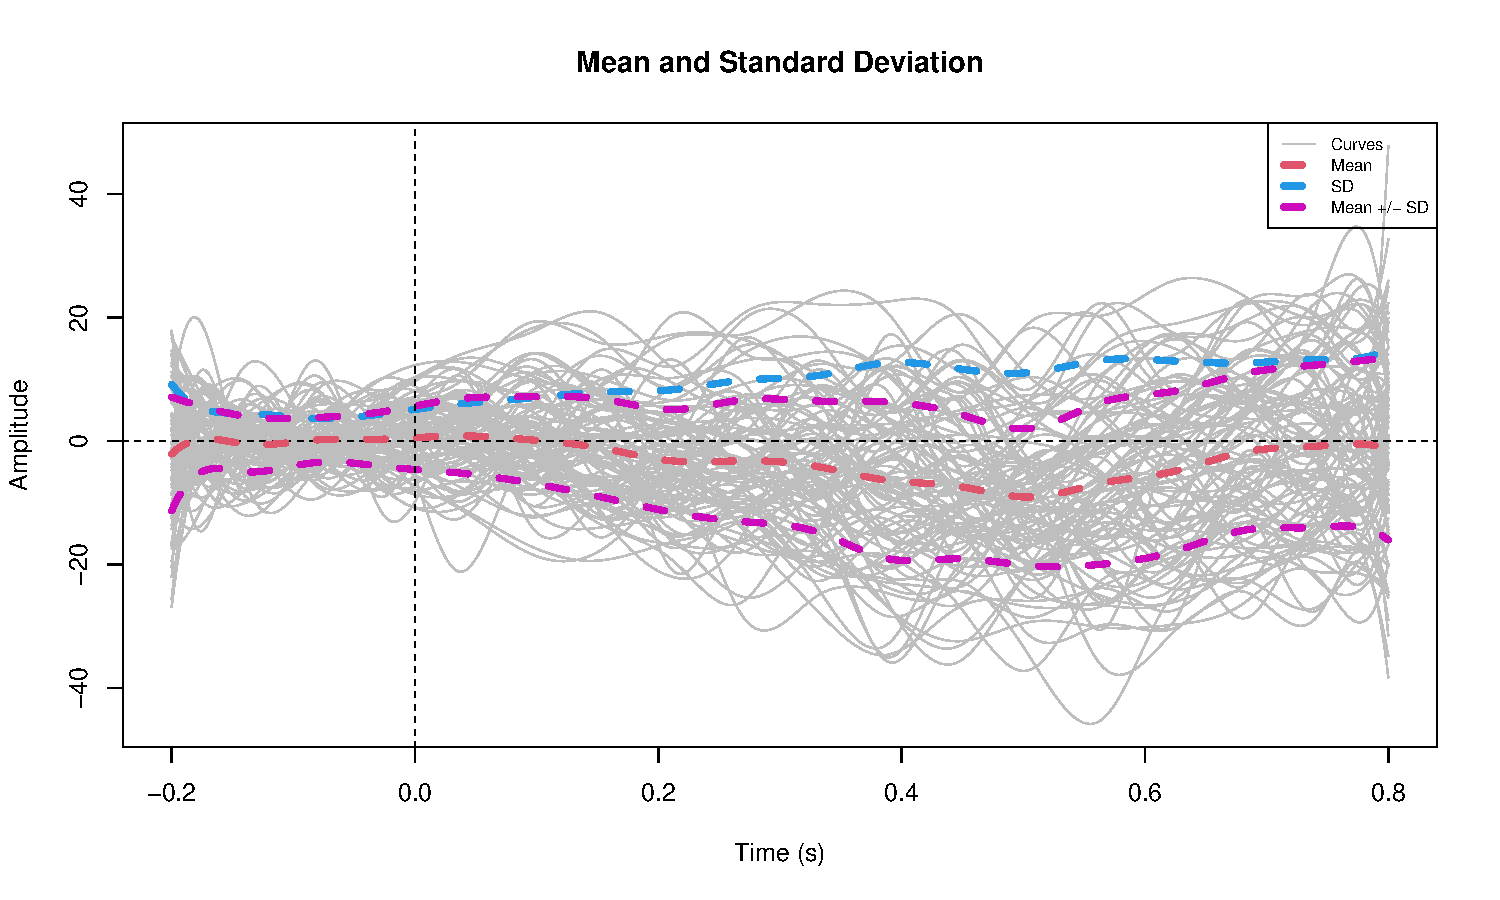
\includegraphics[scale=0.5]{02_mean_sd.pdf}
  \caption{Mean and standard deviation.}
  \label{pic:2}
\end{figure}

% -------------------------------------
\subsection{Covariance}

The sample covariance function quantifies how amplitude values at different time points co-vary
across subjects:

\begin{equation}
  \hat{c}(s,t) = \frac{1}{n-1} \sum_{i=1}^{n}
  \left(x_i(s) - \bar{x}(s)\right) \cdot \left(x_i(t) - \bar{x}(t)\right)
\end{equation}

The resulting bivariate function was visualized using both perspective and image plots. The diagonal
of the covariance surface coincides with the variance function, and the largest values are
concentrated in the time region $0.5$--$0.7\,\mathrm{s}$ on both axes. These results suggest that
the late post-stimulus response constitutes the dominant source of between-subject variability,
whereas the pre-stimulus baseline shows near-zero covariance, indicating consistent behaviour across
subjects during that period.

\begin{figure}[ht]
  \centering
  \begin{subfigure}{0.48\textwidth}
    \centering
    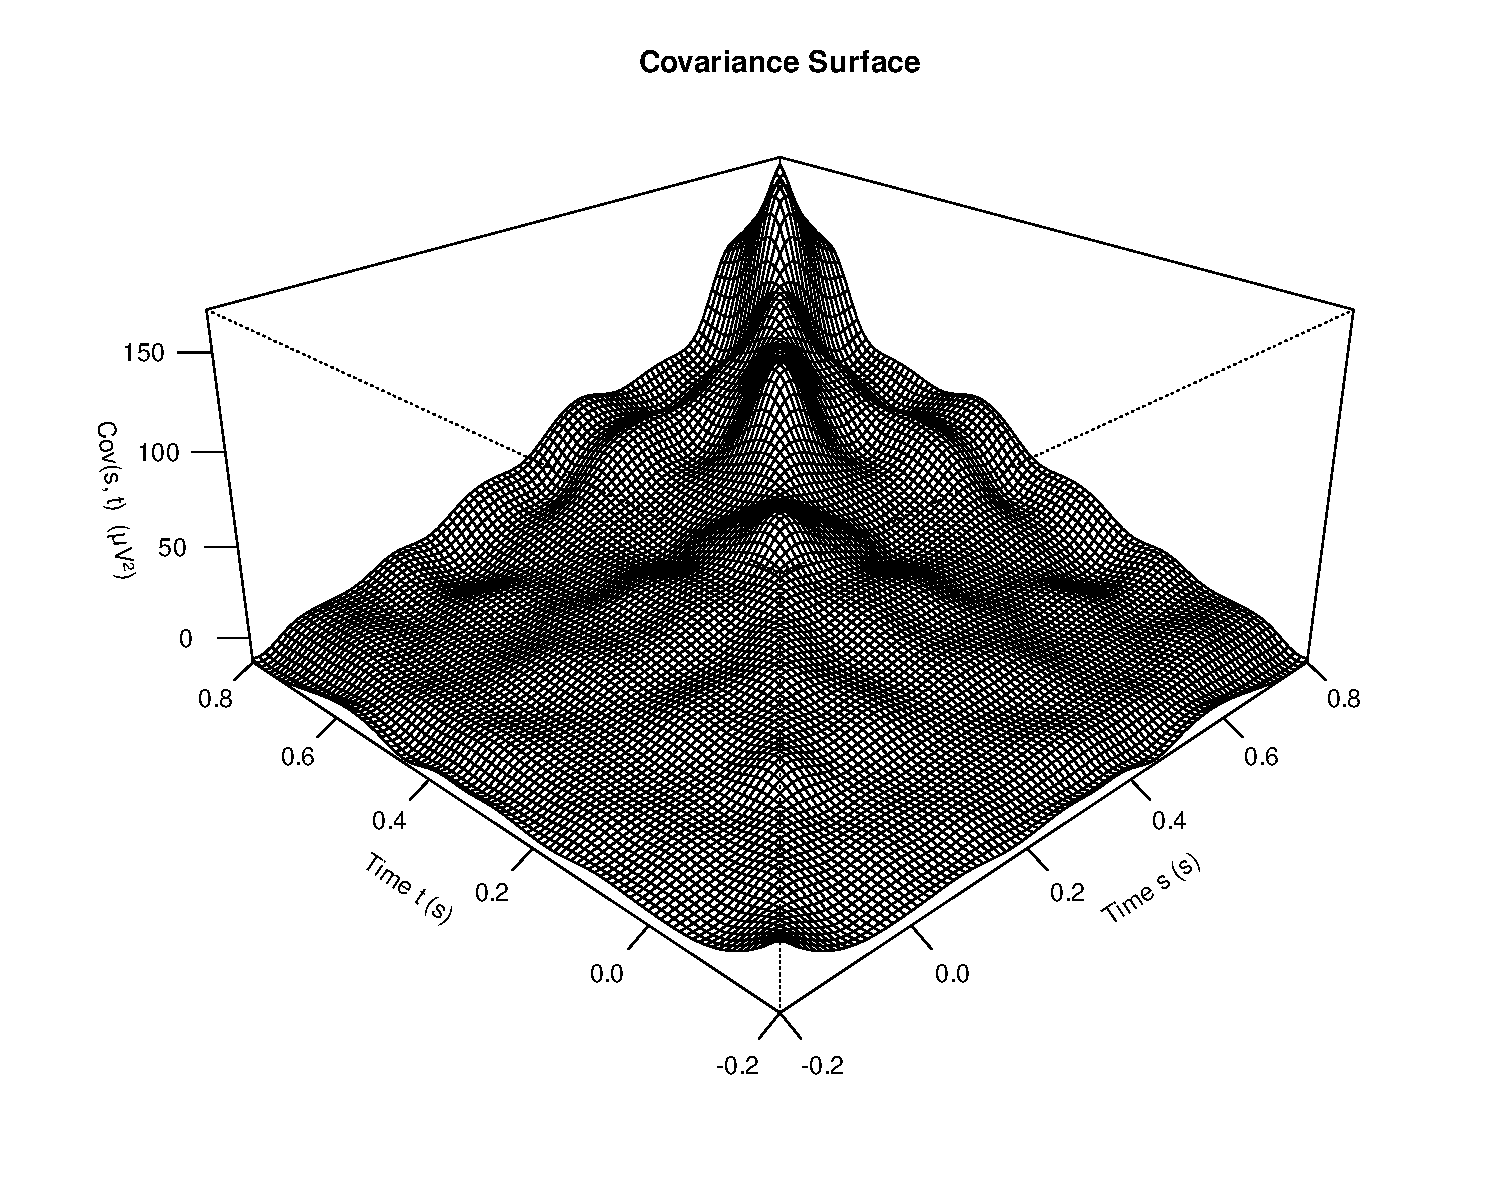
\includegraphics[width=\linewidth]{05_covariance_persp.pdf}
    \caption{Perspective plot}
    \label{fig:left}
  \end{subfigure}
  \hfill
  \begin{subfigure}{0.48\textwidth}
    \centering
    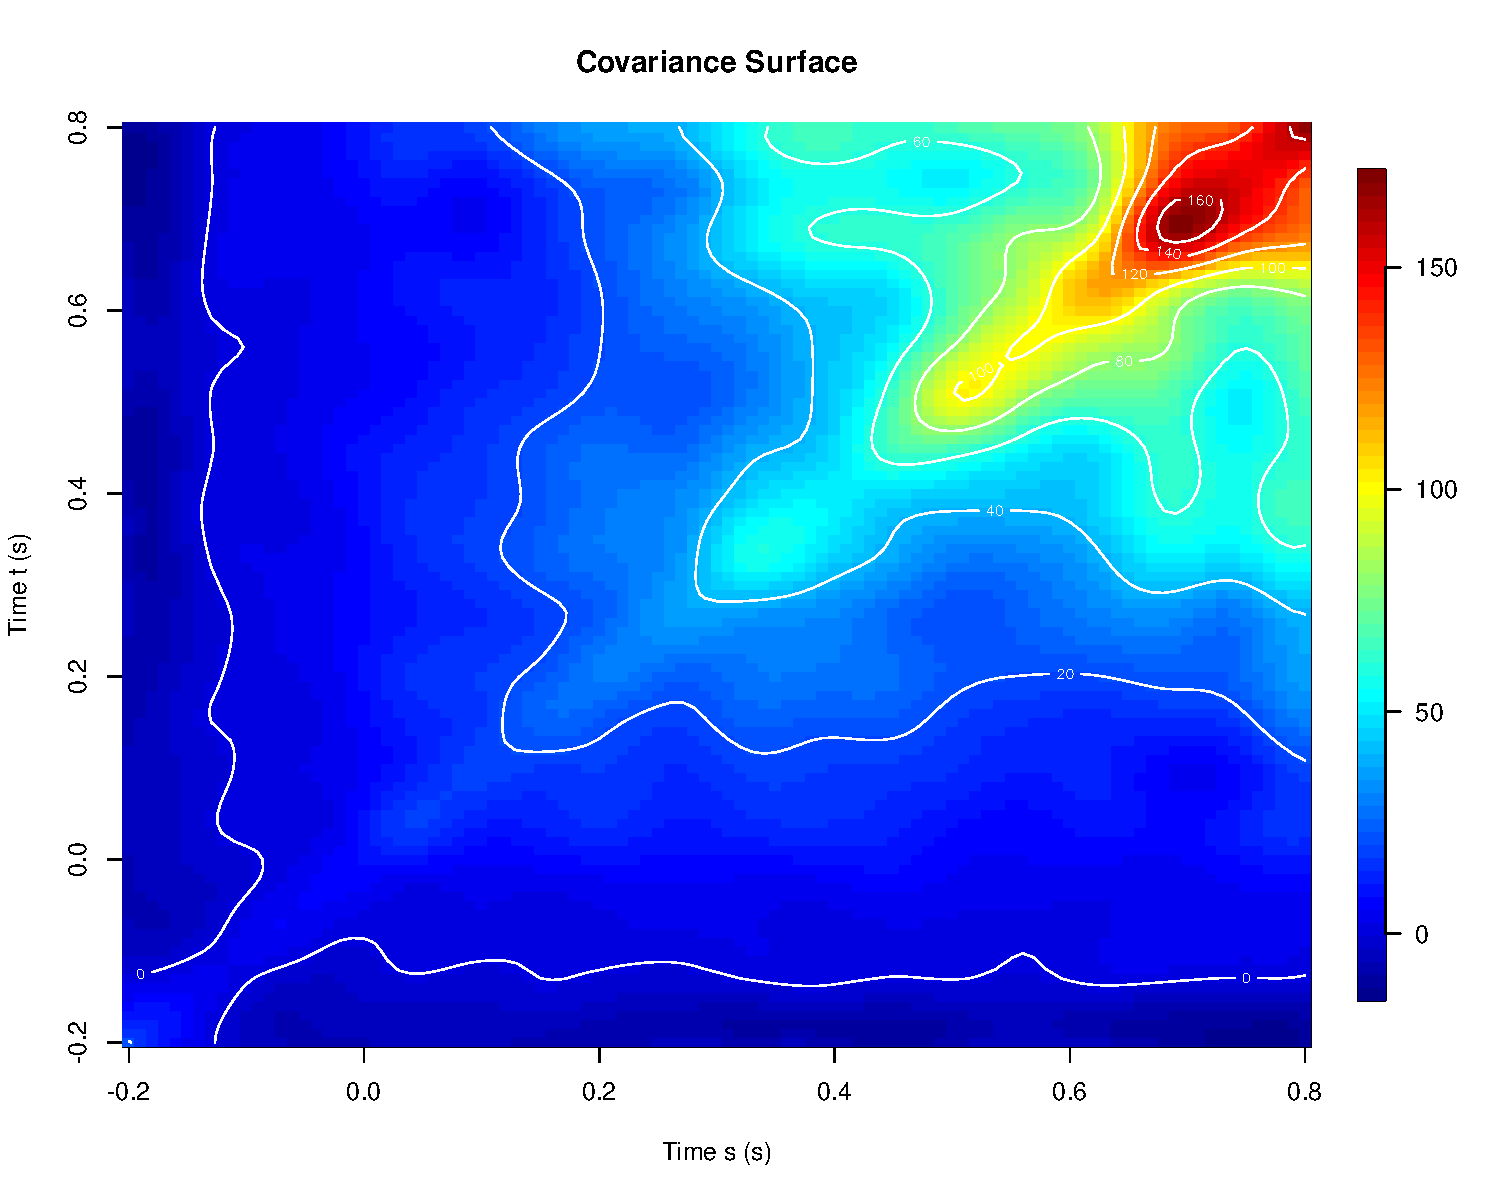
\includegraphics[width=\linewidth]{07_covariance_image.pdf}
    \caption{Image plot}
    \label{fig:right}
  \end{subfigure}
  \caption{Covariance plots}
  \label{fig:both}
\end{figure}

\enlargethispage{1.4\baselineskip}

% -------------------------------------
\subsection{Principal Component Analysis}

Functional Principal Component Analysis (FPCA) was applied to identify the dominant modes of
variation among subjects. The explained variance proportions are:

\begin{itemize}[
  itemsep=5pt,
  topsep=2pt,
  parsep=0pt,
  partopsep=0pt
]
  \item PC1: 61.1\%
  \item PC2: 13.6\%
  \item PC3: 11.9\%
  \item PC4: 3.3\%
\end{itemize}

The first three components cumulatively explain 86.6\% of the total variability, indicating that the
functional data can be effectively summarized by a low-dimensional representation.

\begin{figure}[ht]
  \centering
  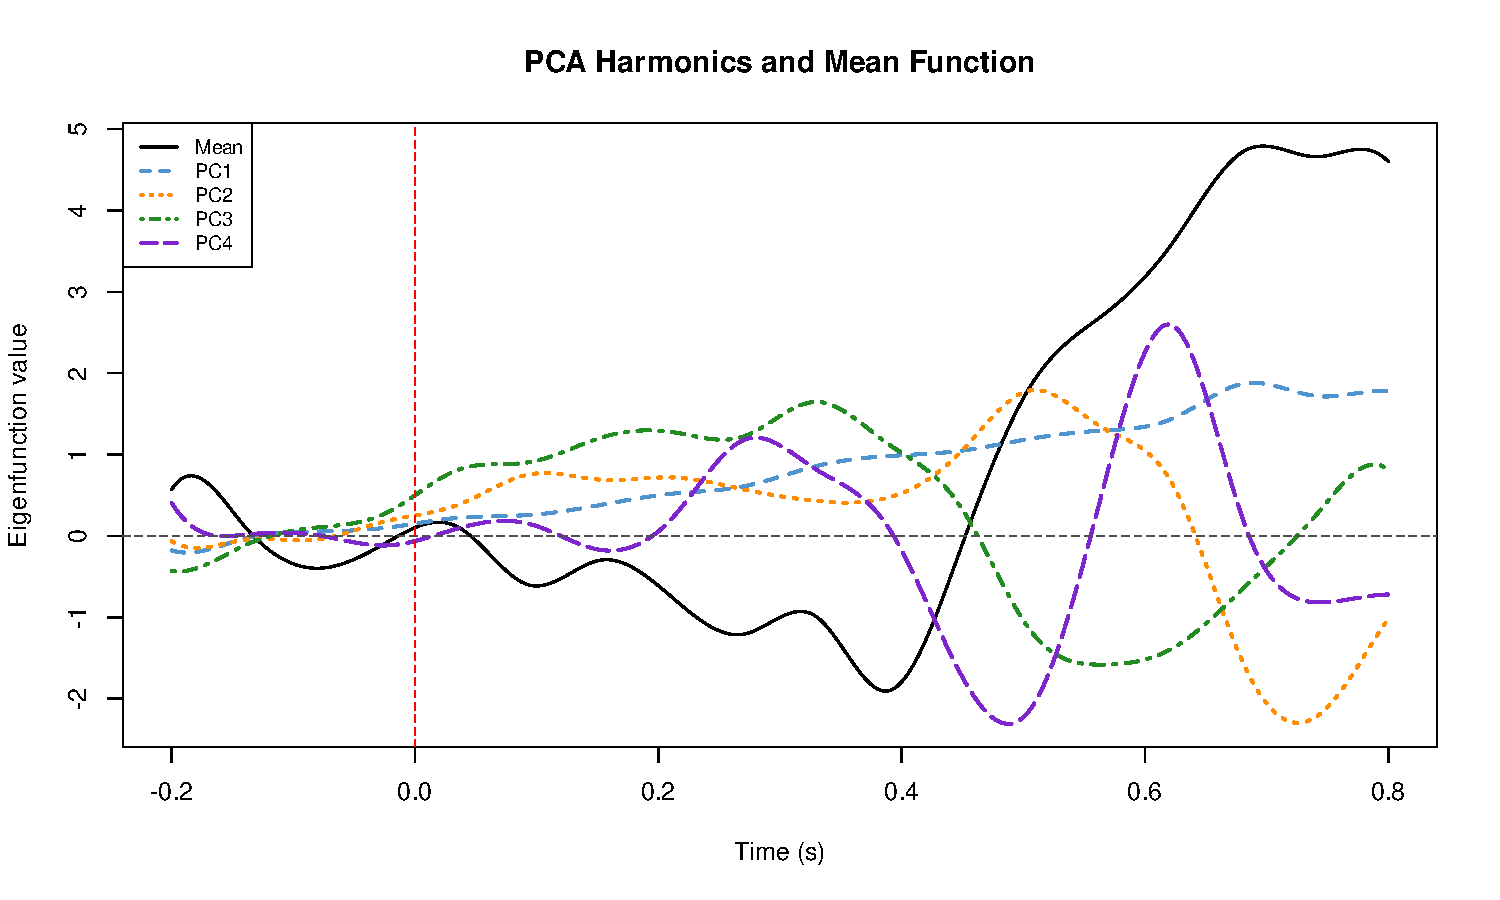
\includegraphics[scale=0.5]{13_pca_harmonics.pdf}
  \caption{PCA harmonics}
  \label{pic:3}
\end{figure}

% -------------------------------------
\subsection{Functional Boxplot}

Functional boxplots based on Modified Band Depth (MBD) and Band Depth (BD2) were used to identify
central and outlying curves. The central 50\% region (analogous to the interquartile range in
classical boxplots), together with the median curve and the fences beyond which curves are flagged
as outliers, were displayed. Both methods identified the same outlier subjects, providing consistent
results.

\begin{figure}[ht]
  \centering
  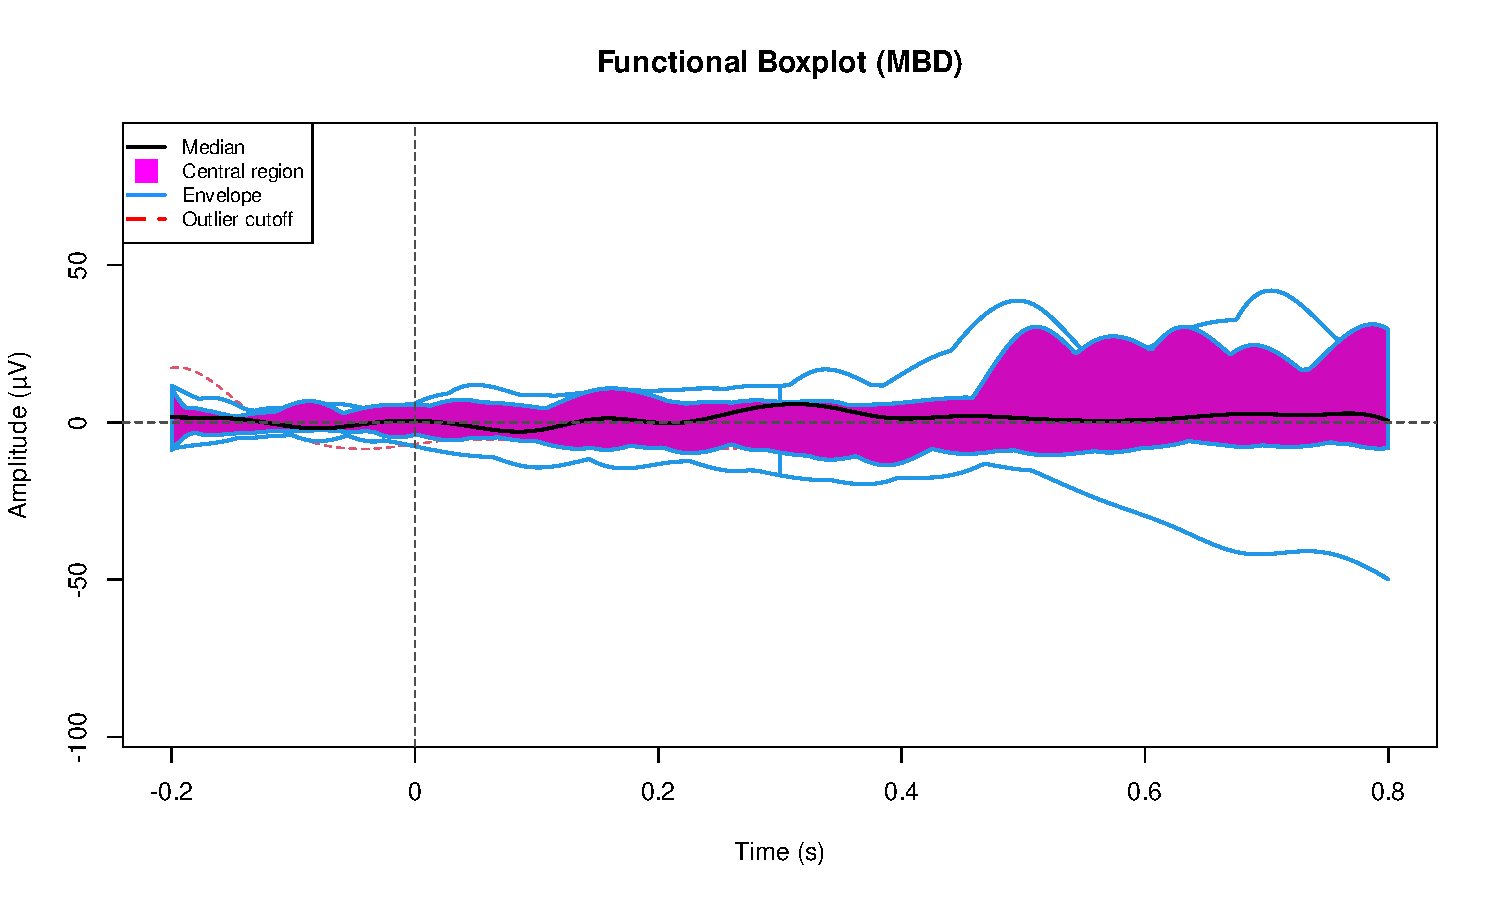
\includegraphics[scale=0.5]{21_fbplot_MBD.pdf}
  \caption{MBD boxplot}
  \label{pic:4}
\end{figure}

% -----------------------------------------------------------------------------
\subsection{Outliers}

Several outlier detection methods were applied, including Highest Density Region (HDR) boxplots and
Massive Unsupervised Outlier Detection (MUOD). Four subjects --- \texttt{sub-003}, \texttt{sub-040},
\texttt{sub-043}, and \texttt{sub-071} --- were identified as outliers by the HDR boxplot at
coverage level $\alpha = (0.05, 0.50)$. All four exhibit substantial negative deflections in the
post-stimulus window: \texttt{sub-071} (purple) shows the most extreme deviation, reaching
approximately $-50~\mu$V after $0.6\,\mathrm{s}$, while \texttt{sub-040} (green) and
\texttt{sub-043} (blue) both descend to about $-20~\mu$V in the same time region. \texttt{sub-003}
(red) shows a less extreme but still atypical negative pattern. These subjects can be classified as
magnitude outliers, as their waveforms have a similar overall shape to the rest of the sample but
are shifted significantly away from the group mean.

\begin{figure}[ht]
  \centering
  
\includegraphics[scale=0.5]{32_hdr_functional_005.pdf}
  \caption{HDR functional boxplot}
  \label{pic:5}
\end{figure}

% -----------------------------------------------------------------------------
\section{Hypothesis testing}

The objective of this part of the project is to determine whether the EEG response curves during the
Flanker task differ significantly between individuals with ADHD symptoms and those without. The ADHD
classification is based on the World Health Organization Adult ADHD Self-Report Scale (ASRS-V1.1),
included in the original dataset. Of the 62 subjects analyzed in the previous sections, 12 were
classified as having ADHD symptoms, 39 as not having ADHD symptoms, and 11 had missing
classifications and were excluded from this analysis. The hypotheses tested are formulated as:

\begin{align}
  H_0 &: \mu_{\text{ADHD}}(t) = \mu_{\text{non-ADHD}}(t),
         \quad \forall\, t \in [-0.2\,\mathrm{s},\, 0.8\,\mathrm{s}] \\
  H_1 &: \mu_{\text{ADHD}}(t) \neq \mu_{\text{non-ADHD}}(t),
        \quad \text{for some } t
\end{align}

% -----------------------------------------------------------------------------
\subsection{Group Comparison}

The 62 smoothed EEG curves were divided into two functional samples according to ADHD
classification. The ADHD group consists of 12 subjects, while the non-ADHD group consists of 39
subjects. Visual inspection of the two groups reveals broadly similar patterns of variability around
the group mean. Both groups exhibit relatively flat behavior during the pre-stimulus baseline and
increased variability in the post-stimulus window.

\begin{figure}[ht]
  \centering
  
\includegraphics[scale=0.5]{HT_01_group_comparison.pdf}
  \caption{Group comparison}
  \label{pic:6}
\end{figure}

The mean functions of the two groups were computed separately and overlaid for comparison. The
non-ADHD mean curve (blue) shows a sustained positive shift after $0.4\,\mathrm{s}$, peaking at
approximately $+6~\mu$V around $0.7\,\mathrm{s}$. The ADHD mean curve (red) follows a similar shape
but with a smaller amplitude in the post-stimulus window, reaching approximately $+4~\mu$V.

\begin{figure}[ht]
  \centering
  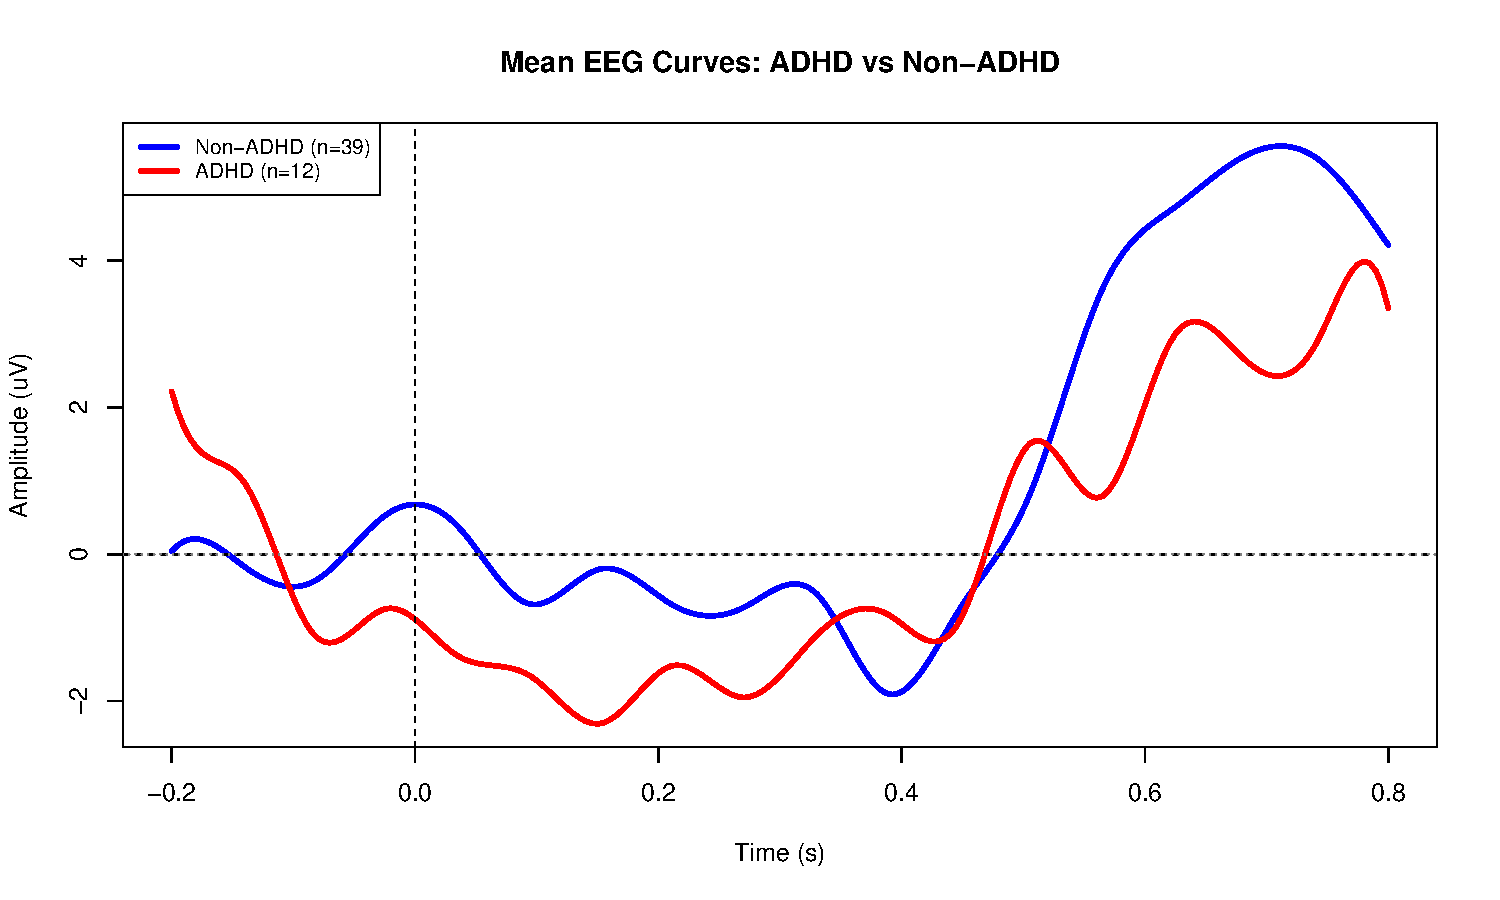
\includegraphics[scale=0.5]{HT_02_mean_comparison.pdf}
  \caption{Mean comparison}
  \label{pic:7}
\end{figure}

% -----------------------------------------------------------------------------
\subsection{Results and Conclusion}

Hypothesis tests were applied to assess whether the two group mean functions differ significantly.
The results are summarized in the table below:

\begin{table}[ht]
  \centering
  \begin{tabular}{lc}
    \toprule
    \textbf{Test} & \textbf{p-value} \\
    \midrule
    Pointwise Z-test ($\max |Z| = 0.66$) & --- \\
    $L^2$-norm test (naive)              & 1.0000 \\
    $L^2$-norm test (bootstrap)          & 0.7260 \\
    F-type test (naive)                  & 1.0000 \\
    F-type test (bootstrap)              & 0.7140 \\
    Permutation test                     & 0.5250 \\
    \bottomrule
  \end{tabular}
  \caption{Summary of hypothesis test results for ADHD vs.\ non-ADHD group comparison.}
  \label{tab:hypothesis_tests}
\end{table}

All tests fail to reject the null hypothesis at the significance level $\alpha = 0.05$. Based on
this analysis, there is no statistically significant difference between the EEG response curves of
individuals with and without ADHD symptoms during the Flanker task at electrode channel FC1.

In addition to the ADHD comparison, hypothesis tests were performed for gender (female vs.\ male)
and socioeconomic status (SES). For the gender comparison, the female group consisted of 37 subjects
and the male group of 25 subjects. For the SES comparison, subjects were grouped into low (SES 1--3,
$n=17$), mid (SES 4--6, $n=29$), and high (SES 7--9, $n=15$) categories, with one subject excluded
due to missing SES data. The results are summarised in Tables~\ref{tab:gender_tests}
and~\ref{tab:ses_test}.

\begin{table}[ht]
  \centering
  \begin{tabular}{lc}
    \toprule
    \textbf{Test} & \textbf{p-value} \\
    \midrule
    Pointwise Z-test ($\max |Z| = 2.50$) & --- \\
    $L^2$-norm test (naive)              & 0.9931 \\
    $L^2$-norm test (bootstrap)          & 0.2600 \\
    F-type test (naive)                  & 0.9926 \\
    F-type test (bootstrap)              & 0.2680 \\
    Permutation test                     & 0.1050 \\
    \bottomrule
  \end{tabular}
  \caption{Hypothesis test results for female vs.\ male group comparison.}
  \label{tab:gender_tests}
\end{table}

\begin{table}[ht]
  \centering
  \begin{tabular}{lc}
    \toprule
    \textbf{Test} & \textbf{p-value} \\
    \midrule
    Functional one-way ANOVA (bootstrap, 500 replications) & 0.4020 \\
    \bottomrule
  \end{tabular}
  \caption{Hypothesis test results for SES group comparison (low/mid/high).}
  \label{tab:ses_test}
\end{table}

All tests fail to reject the null hypothesis at $\alpha = 0.05$. There is no statistically
significant difference in EEG response curves between female and male subjects, nor between subjects
of different socioeconomic backgrounds. Notably, the pointwise Z-test for gender identified 29 time
points where $|Z|$ exceeded the critical value of 2.02, suggesting a localised tendency for
differences in the post-stimulus window, though this did not reach global significance.

% -----------------------------------------------------------------------------
\section{Regression}

To further investigate the relationship between EEG response curves and subject characteristics, we
applied the following regression model:

\begin{equation}
  Y_i(t) = \beta_0(t) + \beta_1(t) \cdot \text{ADHD}_i + \beta_2(t) \cdot \text{Female}_i +
  \varepsilon_i(t), \qquad t \in [-0.2\,\mathrm{s},\, 0.8\,\mathrm{s}]
\end{equation}

\begin{table}[ht]
  \centering
  \begin{tabular}{cll}
    \toprule
    \textbf{Term} & \textbf{Description} & \textbf{Values} \\
    \midrule

    $Y_i(t)$
    & Smoothed EEG curve of subject $i$ at channel FC1
    & Continuous \\

    $\beta_0(t)$
    & Intercept function (baseline mean response)
    & --- \\

    $\beta_1(t)$
    & Coefficient function for ADHD effect
    & --- \\

    $\beta_2(t)$
    & Coefficient function for gender effect
    & --- \\

    $\text{ADHD}_i$
    & Binary indicator of ADHD symptoms
    & 1 = present, 0 = absent \\

    $\text{Female}_i$
    & Binary indicator of gender
    & 1 = female, 0 = male \\

    $\varepsilon_i(t)$
    & Residual error function of subject $i$
    & --- \\

    $t$
    & Time relative to stimulus onset
    & $t \in [-0.2\,\mathrm{s},\, 0.8\,\mathrm{s}]$ \\

    \bottomrule
  \end{tabular}
  \caption{Description of terms in the regression model.}
  \label{tab:model_terms}
\end{table}

% -----------------------------------------------------------------------------
\subsection{Results and Conclusions}

The model summary indicates that the smooth intercept term $\beta_0(t)$ is highly significant ($p =
0.024$), reflecting the structured shape of the average EEG response over time. The ADHD effect
$\beta_1(t)$ is not significant ($p = 0.842$), consistent with the findings from the hypothesis
testing. The female effect $\beta_2(t)$ is significant ($p = 0.016$), suggesting that gender has a
measurable impact on the EEG response shape at channel FC1. The model achieves an adjusted $R^2 =
0.108$, with approximately $11\%$ of the deviance explained.

\begin{table}[ht]
  \centering

  \begin{tabular}{lrrrr}
    \toprule

    \multicolumn{5}{l}{\textbf{Constant coefficients:}} \\
    \midrule

    & \textbf{Estimate}
    & \textbf{Std. Error}
    & \textbf{t value}
    & \textbf{Pr($>|t|$)} \\

    (Intercept)
    & $-0.7201$
    & $1.0344$
    & $-0.696$
    & $0.486$ \\

    \midrule

    \multicolumn{5}{l}{
      \textbf{Smooth terms \& functional coefficients:}
    } \\
    \midrule

    & \textbf{edf}
    & \textbf{Ref.df}
    & \textbf{F}
    & \textbf{p-value} \\

    Intercept(\texttt{yindex})
    & $10.686$
    & $19.000$
    & $9.299$
    & $0.0237$~* \\

    ADHD(\texttt{yindex})
    & $2.001$
    & $2.378$
    & $0.251$
    & $0.8421$ \\

    Female(\texttt{yindex})
    & $4.498$
    & $4.794$
    & $2.762$
    & $0.0159$~* \\

    \midrule

    \multicolumn{5}{l}{
      Signif. codes:
      0 `***' \;
      0.001 `**' \;
      0.01 `*' \;
      0.05 `.' \;
      0.1 ` ' \;
      1
    } \\

    \midrule

    \multicolumn{3}{l}{$R^2_{\text{adj}} = 0.108$}
    & \multicolumn{2}{l}{Deviance explained $= 11.1\%$} \\

    \bottomrule
  \end{tabular}

  \caption{Summary of the regression model.}
  \label{tab:model_summary}
\end{table}

The intercept $\beta_0(t)$ starts at negative values during the pre-stimulus baseline, dips slightly
after stimulus onset, and rises to a peak around $0.5\,\mathrm{s}$. The ADHD coefficient
$\beta_1(t)$ fluctuates around zero across the entire time range, visually confirming the
non-significant p-value. The female coefficient $\beta_2(t)$ shows a more negative deflection during
the post-stimulus window, especially between $0.3$ and $0.6\,\mathrm{s}$. This suggests that female
subjects exhibit systematically lower amplitudes.

\begin{figure}[ht]
  \centering
  
\includegraphics[scale=0.5]{REG_02_individual_coefficients.pdf}
  \caption{Coefficients}
  \label{pic:8}
\end{figure}

The observed curves span a wide range from approximately $-20~\mu$V to $+40~\mu$V with substantial
individual variability, while the fitted curves are restricted to roughly $-6$ to $+6~\mu$V. This
visible reduction in range illustrates the low $R^2$ --- the model captures the average behavior
driven by ADHD and gender but not other factors not included in the model.

\begin{figure}[ht]
  \centering
  
\includegraphics[scale=0.5]{REG_03_fitted_vs_observed.pdf}
  \caption{EEG curves}
  \label{pic:9}
\end{figure}

While ADHD status does not significantly affect the EEG response curve, gender shows a statistically
significant influence, particularly in the post-stimulus window between $0.3$ and $0.6\,\mathrm{s}$.
The relatively low explanatory power of the model ($R^2 \approx 0.11$) suggests that additional
individual-level factors not included in this analysis contribute substantially to the observed
variability in EEG responses.

% -----------------------------------------------------------------------------
\section{Conclusion}

This project applied a complete Functional Data Analysis pipeline to EEG data recorded during a
Flanker cognitive task at electrode channel FC1, using data from 62 young adults from the publicly
available Cognitive Electrophysiology in Socioeconomic Context dataset. In the smoothing step, raw
discrete EEG observations were converted into smooth functional objects using a penalized B-spline
basis expansion with 20 cubic basis functions. The exploratory data analysis revealed that
between-subject variability is concentrated in the post-stimulus window ($0.4$--$0.8\,\mathrm{s}$),
with the first three functional principal components explaining $86.6\%$ of the total variance.
Outlier detection methods consistently identified a small number of subjects classified as magnitude
outliers.

The hypothesis testing procedures investigated whether the mean EEG curves differ between subjects
grouped by ADHD status, gender, and socioeconomic status. For the ADHD and gender comparisons, four
complementary tests were applied: the pointwise Z-test, $L^2$-norm test (naive and bootstrap),
F-type test (naive and bootstrap), and permutation test. For the three-group SES comparison, a
functional one-way ANOVA was used. All tests consistently failed to reject the null hypothesis at
$\alpha = 0.05$, suggesting no statistically significant global differences between any of the
groups.

The functional regression analysis extended these findings by simultaneously modeling the effects of
ADHD status and gender on the EEG curves. ADHD status had no significant effect ($p = 0.842$),
confirming the hypothesis testing results. However, gender showed a statistically significant effect
($p = 0.016$), with female subjects exhibiting systematically lower amplitudes in the post-stimulus
window between $0.3$ and $0.6\,\mathrm{s}$. The relatively low explanatory power of the model ($R^2
\approx 0.11$) suggests that substantial individual variability remains unexplained by the included
covariates.

Overall, the project illustrates how FDA methods can be applied to electrophysiological data to
extract meaningful insights about functional structure, variability, and covariate effects.

\bibliography{samplebib}

\end{document}
